\documentclass[25pt, a0paper, portrait, dvipsnames, innermargin=5mm, innerblockmargin=1cm, blockverticalspace=5mm, colspace=8mm]{tikzposter}
\usepackage[english]{babel}
%\usepackage[style=authoryear, language=english, backend=biber]{biblatex}
\usepackage{xcolor}
\usepackage{hyperref}
\usepackage{enumitem}
\usepackage{amssymb}
\usepackage{tikz}
\usetikzlibrary{shadows}
\usepackage{blindtext}
\usepackage{comment}
\usepackage[justification=centering]{caption}
\usepackage{subfigure}
% tickztable
\newcounter{tablecounter}
%% #1 Caption
\newenvironment{tikztable}[1][]{%
  \def \rememberparameter{#1}%
  \refstepcounter{tablecounter}%
  \vspace{10pt}
  \begin{center}
    \ifx\rememberparameter\@empty
    \else %nothing
    {\small Tab.~\thetablecounter: \rememberparameter \par\medskip} 
    \fi
  }{
  \end{center}
}
\newcommand*{\MyShadow}{\tikz \draw [baseline, fill=ForestGreen,draw=ForestGreen,circular drop shadow] circle (2pt);}
\newcommand*{\MyBall}{\tikz \draw [baseline, ball color=ForestGreen, draw=ForestGreen] circle (3pt);}

% Long title 
\makeatletter
\def\title#1{\gdef\@title{\scalebox{\TP@titletextscale}{%
\begin{minipage}[t]{0.7\linewidth}
\centering
#1
\par
\vspace{0.2em}
\end{minipage}%
}}}
\makeatother

\definecolor{paletaupe}{rgb}{0.74, 0.6, 0.49}
\definecolor{drab}{rgb}{0.59, 0.44, 0.09}
\definecolor{ecru}{rgb}{0.76, 0.7, 0.5}
\definecolor{darktan}{rgb}{0.57, 0.51, 0.32}
\definecolor{forestgreen(web)}{rgb}{0.4, 0.73, 0.09}
\title{Mapping tree communities in tropical forests using joint species distribution models}
\author{ \Large{Jeanne Clément}, \large{UMR AMAP, CNRS}, \texttt{jeanne.clement16@laposte.net} \\ \Large{Ghislain Vieilledent}, \large{UMR AMAP, CIRAD, \texttt{ghislain.vieilledent@cirad.fr}} \vspace{-20mm}}

\usetheme{Envelope}
\usecolorpalette{GreenGrayViolet}
\usecolorstyle[colorPalette=GreenGrayViolet, colorOne=OliveGreen, colorTwo=SpringGreen, colorThree=forestgreen(web)]{Russia}
\colorlet{backgroundcolor}{drab}
\colorlet{innerblocktitlebgcolor}{LimeGreen}
%\usebackgroundstyle{VerticalGradation}
%\addbibresource{biblio-jSDM.bib}
\begin{document}


\maketitle[titletoblockverticalspace=7mm, titletotopverticalspace=-10mm]

\block[bodyinnersep=7mm]{Introduction}
{
Species distribution models (SDMs) are commonly used in ecology to predict the ecological niche of species. However SDMs do not take into account interactions between species to estimate species distributions. Joint Species Distribution Models (JSDMs), which have recently emerged in ecology, allow to take into account co-occurrences between species to predict their distribution. Moreover this approach provides a conceptual framework for integrating functional traits to explain differences in occurrence between species. Many libraries for fitting JSDMs have been developed, but they have some limitations such as supporting large datasets in a reasonable amount of time. Therefore, we have implemented the jSDM R package, which aims to overcome these limitations. }

\begin{columns}
    \column{0.32}
    \block[bodyinnersep=8mm]{Structure of JSDMs}{
      \vspace{-5mm}
    \innerblock{Data used}{    
    \begin{minipage}[c]{0.49\linewidth}
    \begin{tikzfigure}[Data used for fitting JSDMs.]
        \includegraphics[width=0.93\textwidth]{images/dataset}
        \label{fig:dataset}
    \end{tikzfigure}
    \end{minipage}
    \begin{minipage}[c]{0.5\linewidth}
    \begin{itemize}[label={\MyBall}]
        \item $Y$: occurrences of species recorded in a set of spatial sampling units. 
        \item $X$: environmental covariates measured over the sampling units. 
        \item  $T$: traits measured for the species in the $Y$ matrix.
    \end{itemize}
    \end{minipage}
    }
    \vspace{0.6cm}
    \innerblock{Model definition}{
\vspace{1mm}
%According to the article \cite{Warton2015},
We consider that:
\begin{itemize}[label={\MyBall}]
\item $\color{blue}{y_{ij}} \color{black}{ \sim \mathcal{B}inomial(\color{blue}{n_i} , \color{red}{\theta_{ij}}\color{black}{)}}$, for presence-absence data,
\item $\color{blue}{y_{ij}} \color{black}{\sim\mathcal{P}oisson(\color{red}{\theta_{ij}}\color{black}{)}}$, for abundance data, such that:
\vspace{1mm}
    \begin{equation}
     g(\color{red}{\theta_{ij}}\color{black}{)} = \color{red}{\alpha_i} \ \color{black}{+} \ \color{blue}{X_i}\color{red}{\beta_j} \ \color{black}{+} \ \color{red}{W_i\lambda_j}
    \end{equation}
\begin{itemize}[label={\MyBall}]
\vspace{-12mm}
    \item $g$: a link function (probit, logit or log).
    \item $ \color{blue}{n_i}$: number of visits to site $i$.
    \item $ \color{red}{\theta_{ij}}$: occurence probability or mean \\ abundance of species $j$ at site $i$.
    \item $\color{red}{\alpha_i}$: site effect for the site $i$,\\
    if it is a random effect $\color{red}{\alpha_i} \color{black}{\sim \mathcal{N}(0,}\color{red}{V_{\alpha}}\color{black}{)}$, 
    \item  $\color{red}{\beta_j}$: species effect for the species $j$,\\
    if $n$ species traits are considered:\\
    $\color{red}{\beta_j} \color{black}{\sim \mathcal{N}_{p+1}(}\color{red}{\mu_{\beta_j}}\color{black}{,V_{\beta})}$,\\
    with $\color{red}{\mu_{\beta_{jk}}} \color{black}{ = \sum_{r=0}^{n}} \ \color{blue}{t_{jr}}.\color{red}{\gamma_{rk}}$, for $k\in[0,p]$,\\ considering $p$ covariates and the intercept.
    \item $\color{red}{\lambda_j}$: factor loadings for species $j$.
    \item $\color{red}{W_i}$: latent variables (or "unmeasured predictors") for site $i$.
\end{itemize}
\end{itemize}
\vspace{-1mm}
This latent variable model (\textbf{LVM}) is equivalent to a \\ particular case of the generalized linear multivariate model (\textbf{GLMM}): 
    \begin{equation}
     g(\color{red}{\theta_{ij}}\color{black}{)} = \color{red}{\alpha_i} \ \color{black}{+} \ \color{blue}{X_i}\color{red}{\beta_j} \ \color{black}{+} \ \color{red}{u_{ij}}
     \vspace{4mm}
    \end{equation}
    such that $\color{red}{u_i} \color{black}{\sim \mathcal{N}_J(0_{\mathbb{R}^J}, }\color{red}{\Sigma}\color{black}{)}$, by assuming $\color{red}{u_{ij}} \color{black}{=} \color{red}{W_i\lambda_j}$, \vspace{1mm} \\
    and $\color{red}{\Sigma_{jg}} \color{black}{=} \color{red}{\lambda_j}\color{black}{^T} \color{red}{\lambda_{g}}$. \vspace{5mm}
\\
The \textbf{full species residual correlation matrix} is then defined as follows:
\vspace{-3mm}
\begin{equation}
  R_{jg}:=\frac{\Sigma_{jg}}{\sqrt{\Sigma _{jj}\Sigma _{gg}}}.
  \end{equation}
  }
  \vspace{-3mm}
 }
\block[bodyinnersep=8mm]{ \vspace{-7mm} R package \texttt{jSDM}
    \makebox[0pt][l]{\hspace*{1mm}\raisebox{-2ex}{\includegraphics[scale=0.55]{images/logo-jSDM.png}}} \qquad \vspace{-6mm}}{
Recently developed \texttt{jSDM} R package for fitting JSDMs:
\vspace{2mm}
\begin{itemize}[label={\MyBall}]
\item Website: \url{https://ecology.ghislainv.fr/jSDM}
\vspace{2mm}
\item Bayesian inference methods according to link function:
\begin{itemize}[label={\MyBall}]
\item Gibbs sampler with conjugate priors (probit),  
\item Metropolis-within-Gibbs algorithm (logit, log).
\end{itemize}
\vspace{1mm}
\item Optimized code to treat large data-sets in limited time:
%to reduce computation time on large data-sets
\begin{minipage}[c]{0.86\linewidth}

\begin{itemize}[label={\MyBall}]
\vspace{0.1cm}
\item R package \texttt{Rcpp} to include C++ code,
\vspace{0.3cm}
\item \texttt{Armadillo} library for matrix calculations, 
\vspace{0.3cm}
\item \texttt{GSL-GNU} scientific library for random draws.
\end{itemize}
\end{minipage}
    \begin{minipage}[c]{0.1\linewidth}
    \vspace{1mm}
    \includegraphics[scale=0.09]{images/logo_Rcpp.png} \vspace{0.1cm} \\ 
    \includegraphics[scale=0.64]{images/logo_Armadillo.png} \vspace{0.1cm} \\
    \includegraphics[scale=0.1]{images/logo_GNU.png}
    \end{minipage}
\vspace{-5mm}
\end{itemize}

}
    \column{0.68}
     \block[bodyinnersep=8mm]{Benchmarking our method against state-of-the-art JSDM implementation}
    {
    We fitted JSDMs of the form: $g(\color{red}{\theta_{ij}}\color{black}{)} = \ \color{blue}{X_i}\color{red}{\beta_j} \ \color{black}{+} \ \color{red}{W_i\lambda_j}$, on 6 real data-sets and a simulated one using: 
    \begin{itemize}[label={\MyBall}]
    \item\texttt{Hmsc} 3.0-11:  R package for Hierarchical Modelling of Species Communities (based on R code).
    \item  \texttt{boral} 2.0:  R package for Bayesian Ordination and Regression Analysis (based on \texttt{JAGS} code).
    \item \texttt{jSDM} 0.2.1 : R package, we have developed (based on Rcpp and C++ compiled code). 
    \end{itemize}
    \begin{minipage}[c]{0.6\linewidth}
    \begin{tikztable}[Comparison of computation times and accuracy of results between the three packages]
            \colorbox{white}{\includegraphics[width=0.93\textwidth]{images/comparison_poster.pdf}}
    \label{fig:comparison}
    \end{tikztable}
    \end{minipage}
    \begin{minipage}[c]{0.4\linewidth}
        \begin{itemize}[label={\MyBall}]
        \item n.col.X, n.traits, n.latent: number of covariates,\\ species traits and latent axes,
        \vspace{5mm}
        \item n.param: parameters to estimate, 
        \vspace{5mm}
        \item n.mcmc number of iterations,
        \vspace{5mm}
        \item RMSE: Root-Mean-Square Error of the occurrence probabilities ($\theta_{ij}$) for the simulated data-set.  %RMSE$=\frac{1}{IJ}\sum\limits_{i=1}^{I}\sum\limits_{j=1}^{J}((\theta_{ij} - \hat{\theta}_{ij})^2$
        \vspace{5mm}
        \item Deviance computed as follows : \\ $D=-2\sum_{i}\sum_{j}\log(\mathbb {P}(y_{ij}\ |\ \hat{\theta}_{ij}))$,
        \vspace{3mm}
        \item TSS: True Skills Statistic,\\  TSS$:=$sensitivity$+$specificity$-1$.
        %considering the lowest estimated probability value for an \\ occurrence point ($\tau_i$), as the presence threshold for the site $i$. 
        \end{itemize}
        \end{minipage}
     \begin{itemize}[label={\MyBall}]
     \vspace{0.3cm}
     \item \texttt{jSDM} is \textbf{2} to \textbf{7} times faster than \texttt{Hmsc} and \textbf{15} to \textbf{439} times faster than \texttt{boral} for presence-absence data-sets.
     \item \texttt{jSDM} is \textbf{1.5} to \textbf{2.1} times faster than \texttt{Hmsc} and \textbf{1.7} to \textbf{2.9} times faster than \texttt{boral} for abundance data-sets. 
     \item \texttt{jSDM} provides either more accurate or equivalent estimates than \texttt{Hmsc} and \texttt{boral}, given the RMSE, TSS and Deviance values. 
     \end{itemize}
    }
    
\block[bodyinnersep=8mm]{Mapping tree communities in Madagascar from large forest inventories}{
\vspace{-2mm}
\begin{minipage}{0.54\linewidth}
    \begin{minipage}[c]{0.66\linewidth}
    \innerblock{Data-sets considered}{
    \begin{itemize}[label={\MyBall}]
    \item National forest inventories (1994-1996).
    \item Climatic variables (1960-1990):
    \begin{itemize}[label={\MyBall}]
    \item Average annual temperature ($ ^ \circ C$),
    \item Average annual precipitation (mm),
    \item Seasonality of temperature,
    \item Seasonality of precipitation,
    \item Annual climatic water deficit (mm).
   \end{itemize}
   \end{itemize}
   }
   \end{minipage}
   \hspace{-1cm}
   \begin{minipage}[c]{0.32\linewidth}
   \innerblock{Residual correlation}{
   \vspace{-2mm}
   \begin{tikzfigure}[\vspace{-3mm}
$R$ estimated between the 25 more abundant species] 
   \vspace{-3mm}
    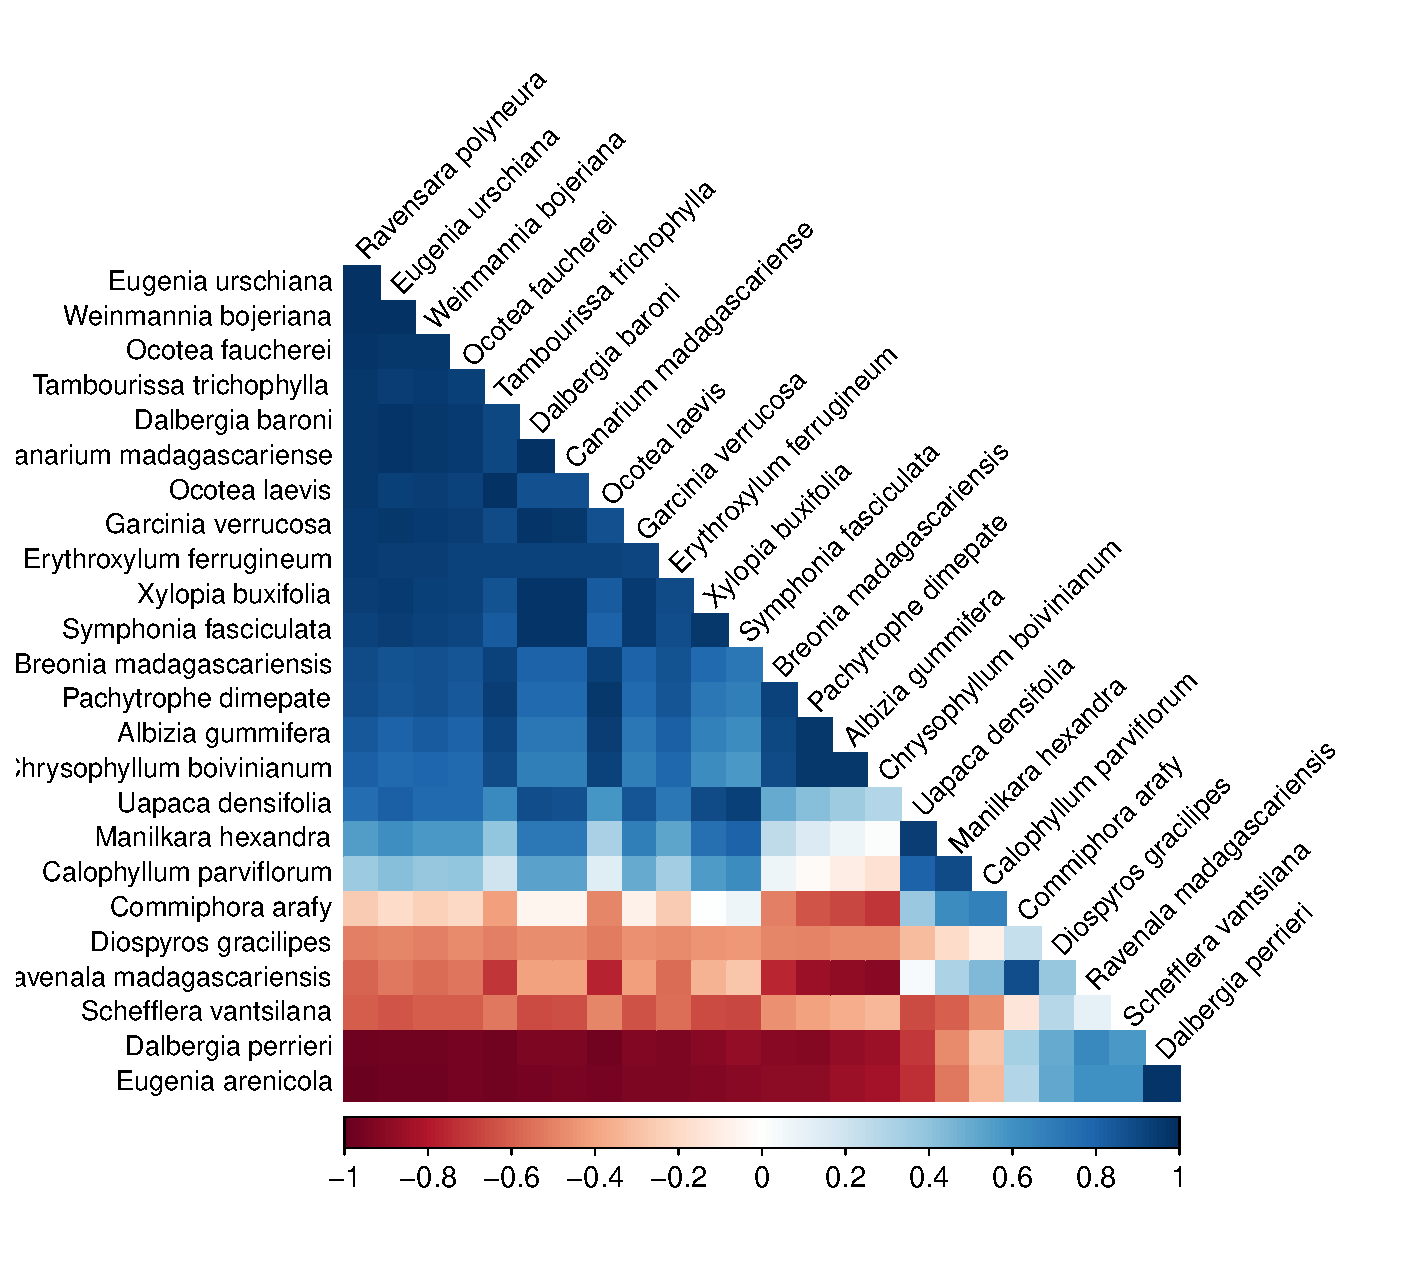
\includegraphics[width=0.91\textwidth]{images/res-corr-poster.eps}
    \vspace{-2cm}
  \end{tikzfigure}
  \vspace{-6mm}
   }
   \end{minipage}
    \vspace{3mm}
   \innerblock{Spatial interpolation of sites' parameters}{
    \begin{minipage}{0.5\linewidth} 
   \begin{itemize}[label={\MyBall}]
   \item Regularized Spline with Tension
   \item Occurrence probabilities \\ $\Rightarrow$ species distribution maps.
   \end{itemize}
   \end{minipage}
   \begin{minipage}{0.5\linewidth}
    \begin{tikzfigure}
    \renewcommand{\thefigure}{3}
    \renewcommand{\figurename}{Fig.}
    \centering
     \begin{minipage}{0.6\linewidth}
     \centering
    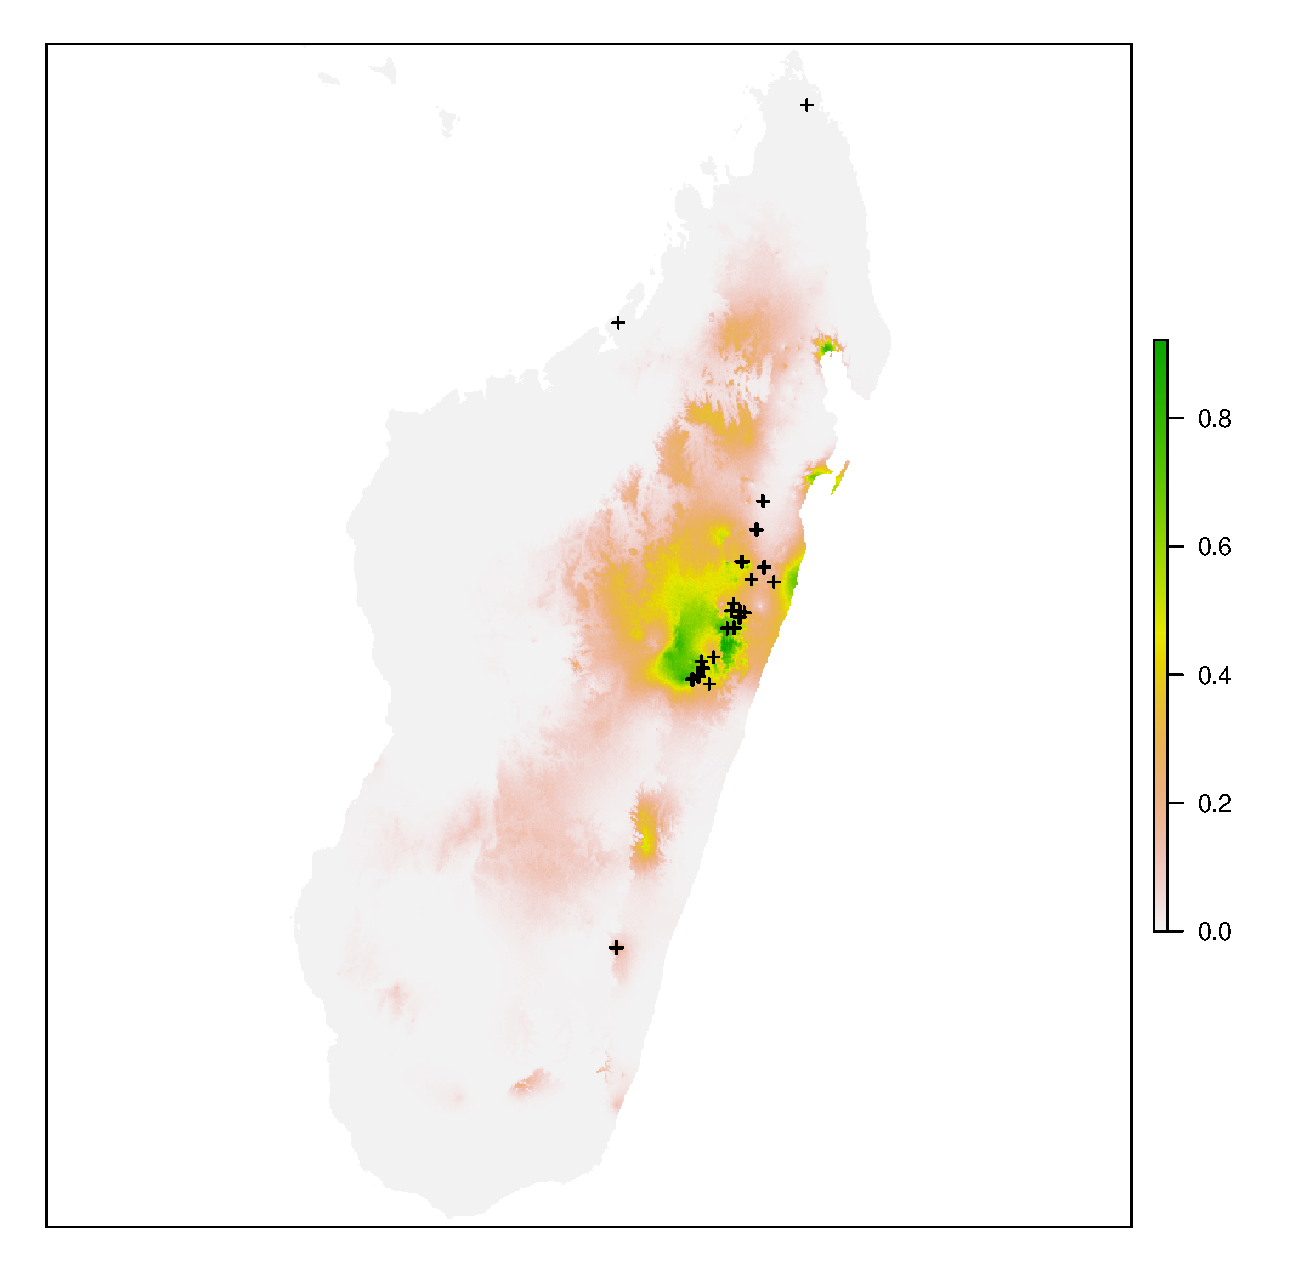
\includegraphics[width=0.8\textwidth]{images/dist_sp1-poster.eps}
    \end{minipage}
    \begin{minipage}{0.35\linewidth}
    \captionsetup{justification=left}
    \captionof{figure}{Ocotea laevis species distribution and occurrences}
    \end{minipage}
    \end{tikzfigure}
   \end{minipage}
   }
   \vspace{3mm}
    \innerblock{Estimated species richness in Madagascar}{
    \vspace{-1mm}
    \begin{itemize}[label={\MyBall}]
    \item Species richness observed at site $i$ defined by $R_i:=\sum_{j}y_{ij}$.
    \vspace{-1mm}
    \item Species richness estimated at site $i$: $\widehat{R}_i=\sum_{j} \hat{\theta}_{ij}$.
    \end{itemize}
   \begin{tikzfigure} 
    \renewcommand{\thefigure}{4}
    \renewcommand{\figurename}{Fig.}
    \captionsetup{justification=centering}
    \centering
    \begin{minipage}{0.25\linewidth} 
        \vspace{-1.6cm}
    \centering
    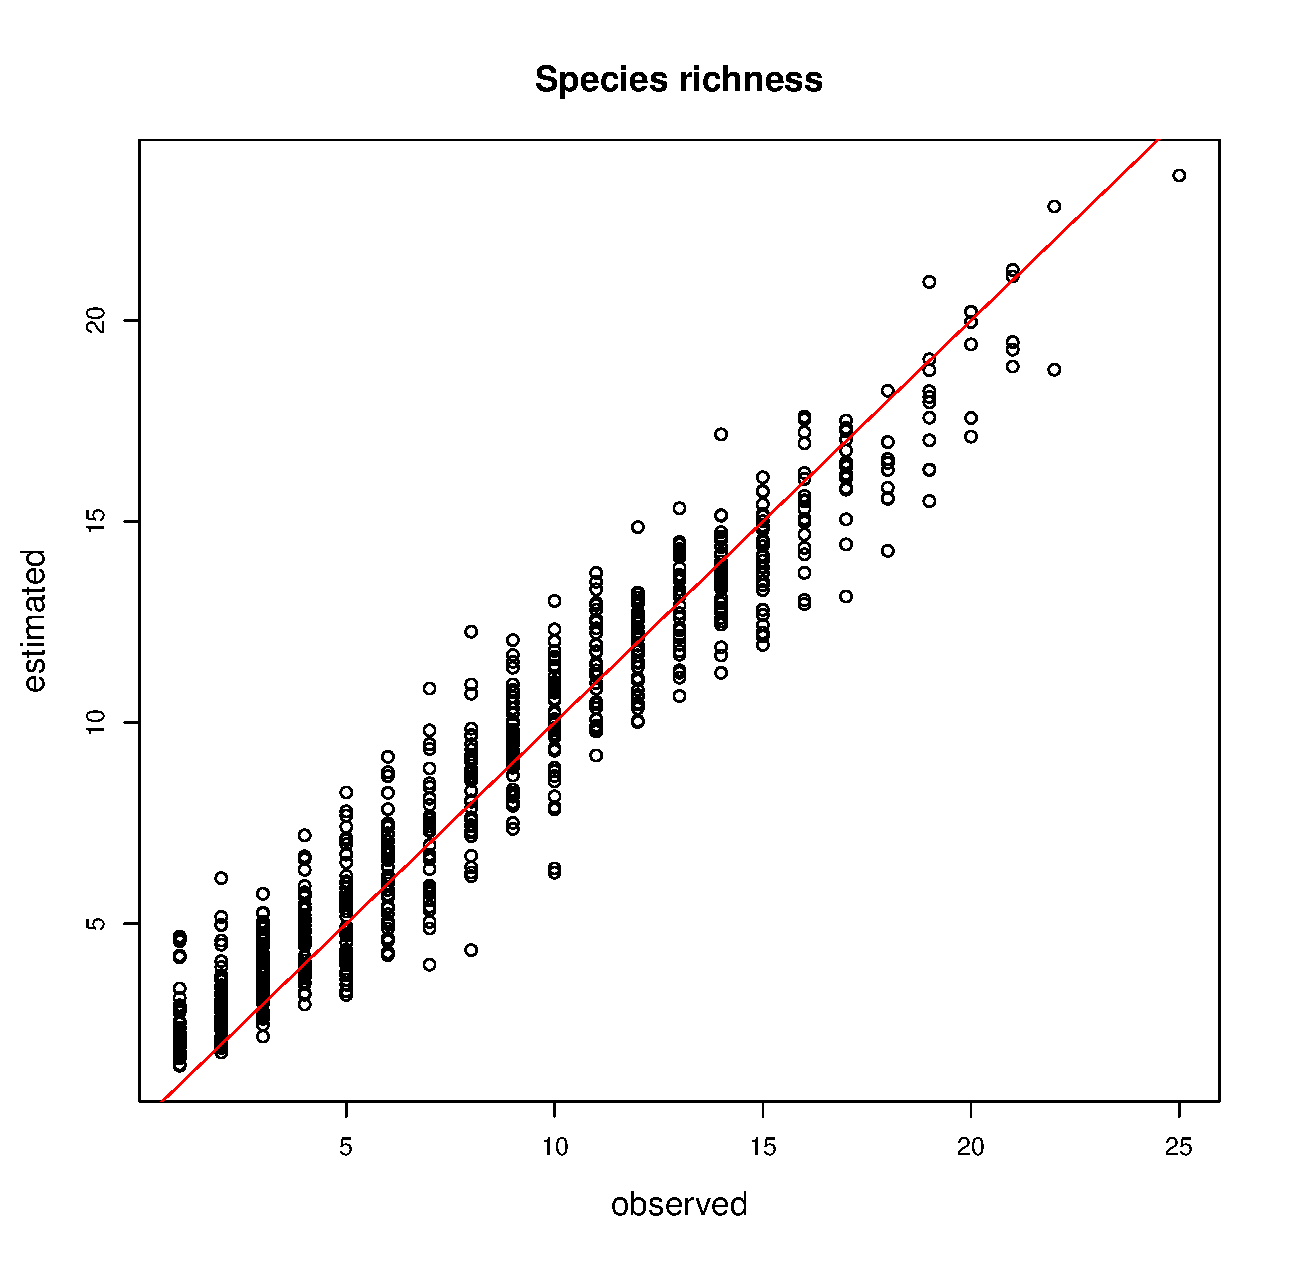
\includegraphics[width=1\textwidth]{images/sp-rich-obs-fitted.eps}
    \captionof{subfigure}{\textit{Species richness estimated and observed at inventory sites.}}
    \label{fig:4a}
    \end{minipage} 
    \begin{minipage}{0.35\linewidth} 
    \centering
    \vspace{-1.7cm}
    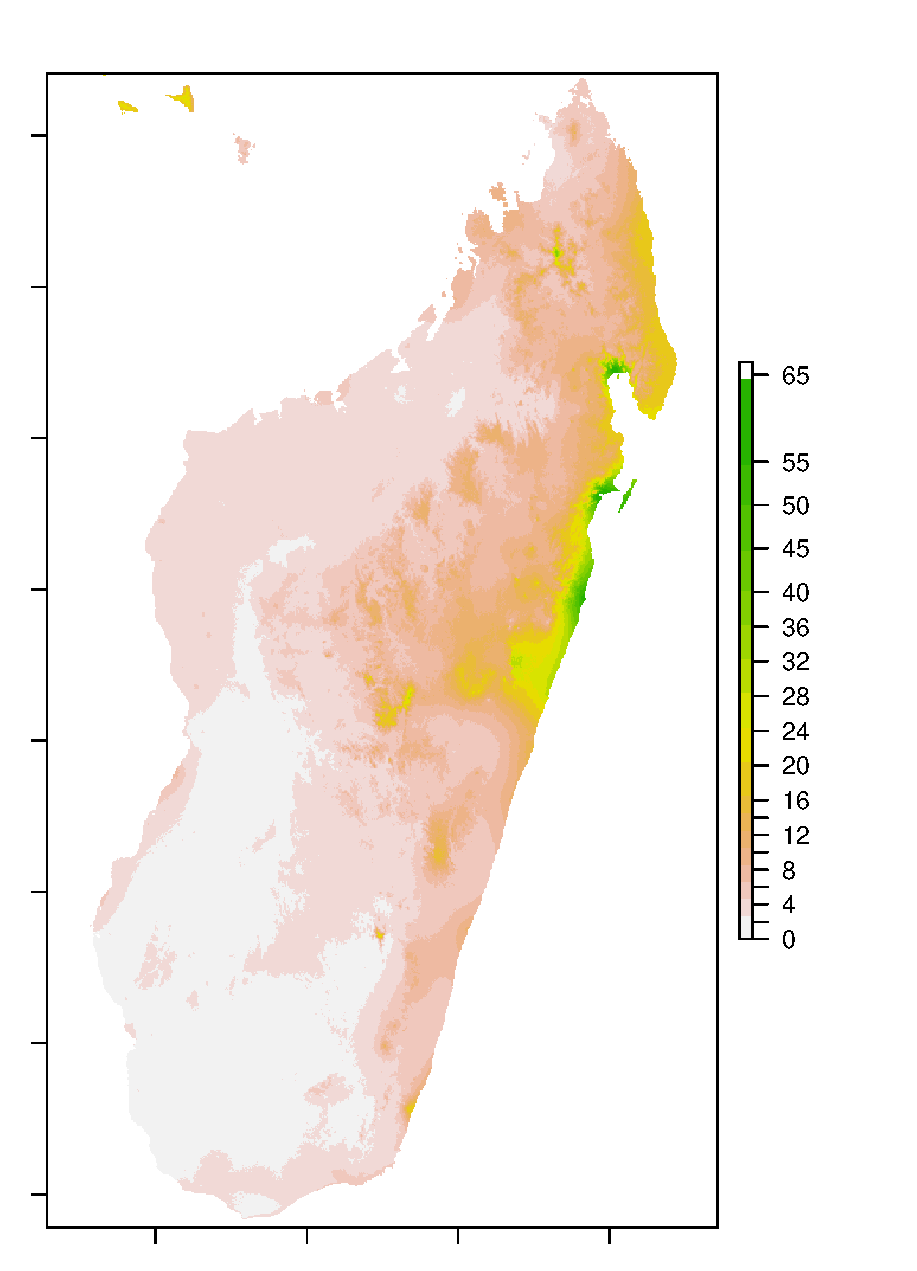
\includegraphics[width=0.65\textwidth]{images/sp-rich-poster.eps}
    \captionof{subfigure}{\textit{Species richness at Madagascar scale.}} 
    \label{fig:4b}
    \end{minipage}
    \begin{minipage}{0.35\linewidth} 
    \vspace{-6mm}
    \centering
    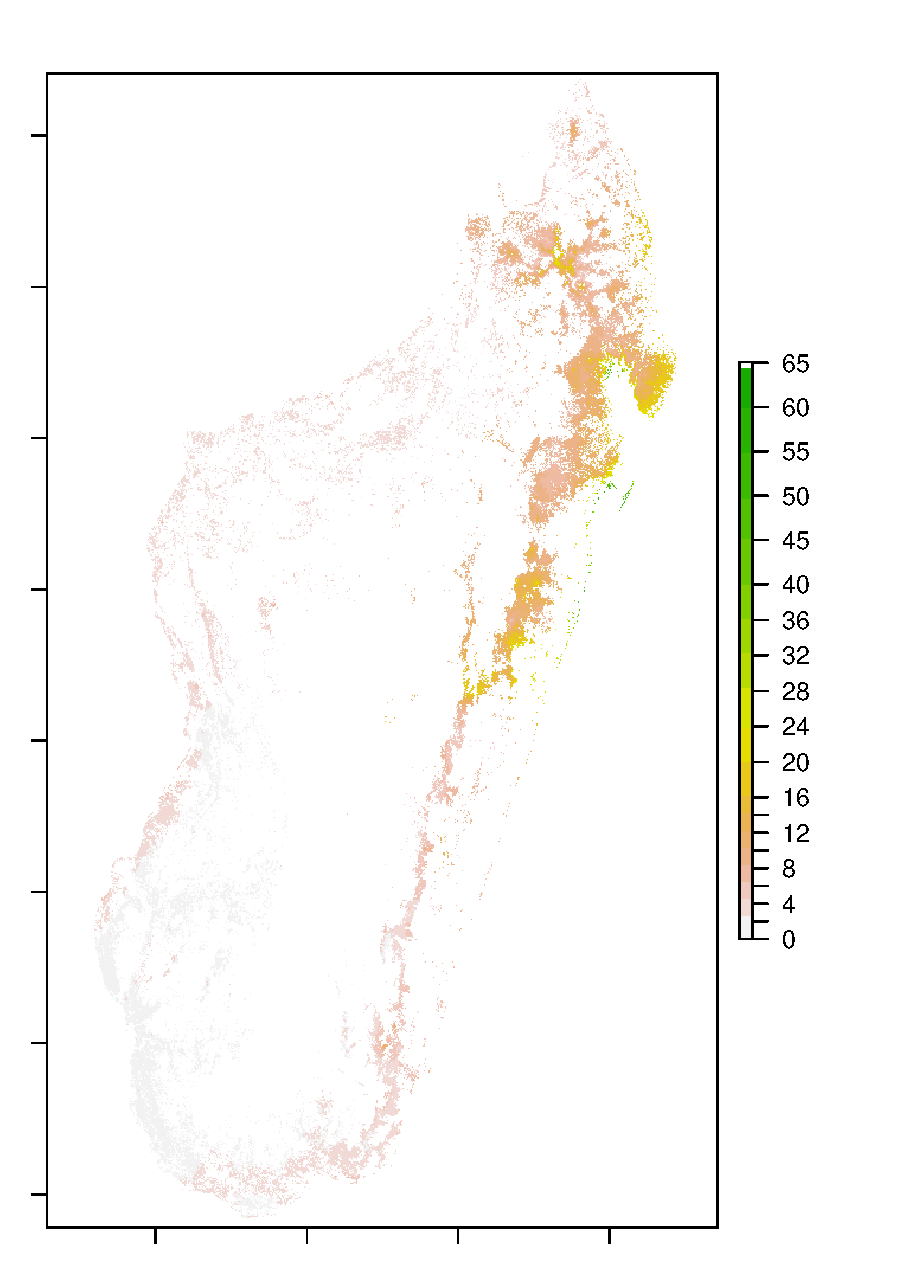
\includegraphics[width=0.65\textwidth]{images/sp-rich-deforest-poster.eps}
    \captionof{subfigure}{\textit{Species richness \\ restricted to forest cover in 2000.}} 
    \vspace{-3mm}
    \label{fig:4c}
    \end{minipage} 
    \captionof{figure}{\textit{Species richness estimated in Madagascar}} 
    \label{fig:4}
    \end{tikzfigure} 
    \vspace{-4mm}}
\end{minipage}
   \hspace{2mm}
   \begin{minipage}[c]{0.45\linewidth}
   \vspace{-3mm}
   \innerblock{Fitting JSDM from Madagascar data-sets}{
   \vspace{3mm}
   We performed, a quadratic binomial regression,  \vspace{2mm} using \\ \texttt{jSDM}, such that: 
   $\textrm{probit}(\color{red}{\theta_{ij}}\color{black}{)} = \ \color{blue}{X_i}\color{red}{\beta_j} \ \color{black}{+} \ \color{red}{W_i\lambda_j} \ \color{black}{+} \ \color{red}{\alpha_i}.$
   \vspace{4mm}
   \begin{tikztable}[Data-sets dimensions, computation time and accuracy of results.]
            \colorbox{white}{\includegraphics[width=0.96\textwidth]{images/JSDM_Mada_poster.pdf}}
    \label{fig:JSDM_Mada}
    \end{tikztable}
    \vspace{-1cm}
   }
   \vspace{5mm}
    \innerblock{Tree species community map in Madagascar}{
    \vspace{4mm}
    Method:
    \vspace{3mm}
    \begin{itemize}[label={\MyBall}]
        \item Normalized PCA on species' occurrence probabilities,
        \vspace{2mm}
        \item Coordinates of the first three axes scaled to [0,255],
        \vspace{2mm}
        \item  \textcolor{red}{R}\textcolor{ForestGreen}{G}\textcolor{blue}{B} coloration of the pixels given their coordinates on the first three axis of the PCA. 
    \end{itemize}
     \vspace{3mm}
    \begin{tikzfigure} 
    \renewcommand{\thefigure}{5}
    \renewcommand{\figurename}{Fig.}
    \centering
    \begin{minipage}{0.31\textwidth} 
    \centering
    \vspace{-2.3cm}
    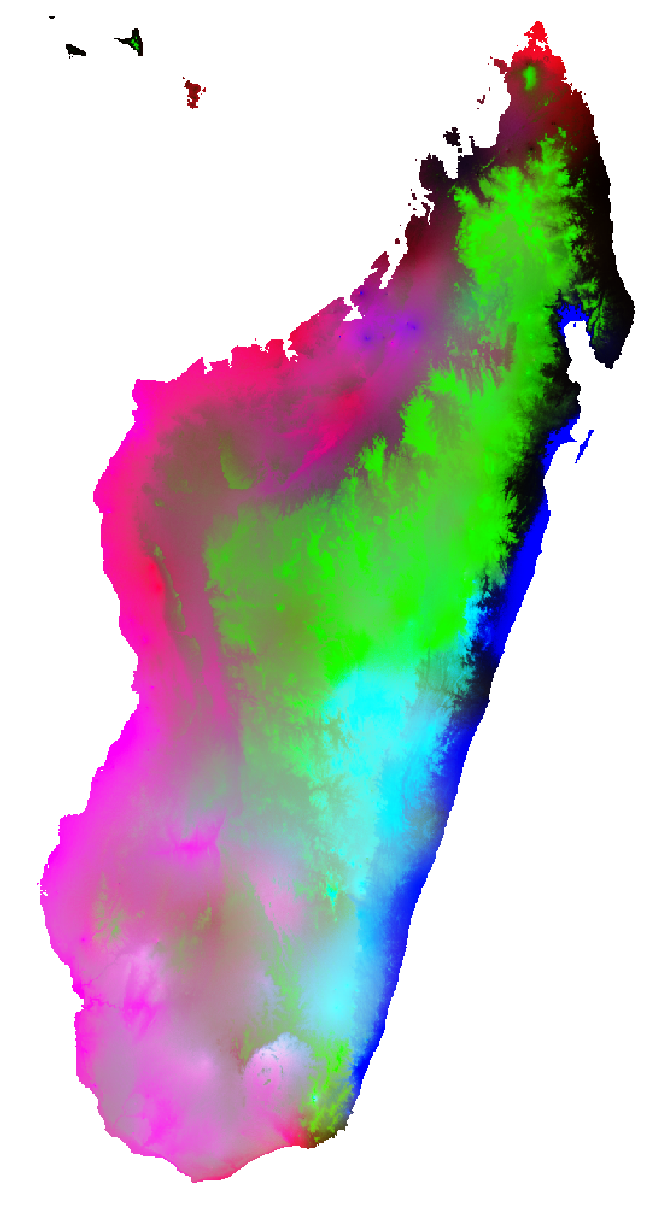
\includegraphics[width=0.7\textwidth]{images/beta-div-poster.eps}
    \captionof{subfigure}{\textit{Species turnover.}} 
    \label{fig:5a}
    \end{minipage}
    \begin{minipage}{0.31\textwidth} 
    \centering
    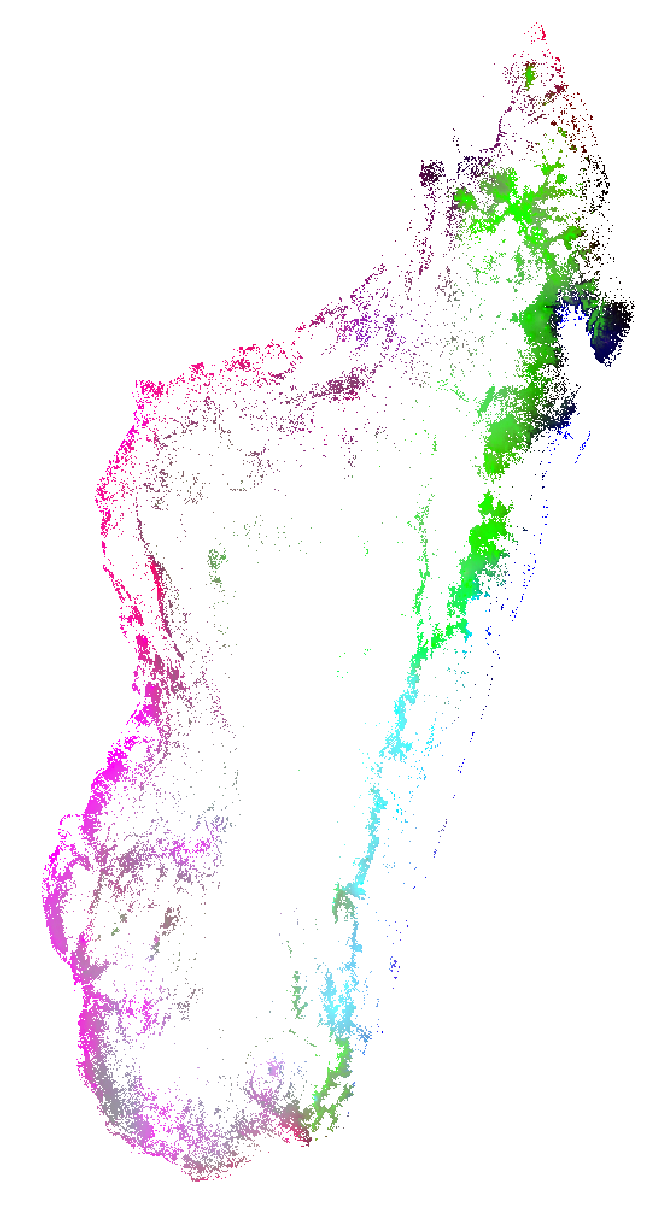
\includegraphics[width=0.7\textwidth]{images/beta-div-deforest-poster.eps}
    \captionof{subfigure}{\textit{Species turnover restricted to forest cover in 2000.}} 
    \label{fig:5b}
    \end{minipage} 
    \begin{minipage}{0.31\textwidth} 
    \vspace{-3cm}
    \centering
    \includegraphics[width=0.7\textwidth]{images/mada_forest_type.jpg}
    \captionof{subfigure}{\textit{Forest types}} 
    \label{fig:5c}
    \end{minipage} 
    \captionof{figure}{\textit{Estimated species turnover and forest types in Madagascar}} 
    \label{fig:5}
    \vspace{2mm}
    \end{tikzfigure} 
    \begin{itemize}[label={\MyBall}]
    \item pixels with $\neq$ colors $\Rightarrow$ species present are not the same. 
    \item pixels with $\simeq$ colors $\Rightarrow$ communities of similar species.
    \end{itemize}
    \vspace{-2mm}
}
   \end{minipage}
 \vspace{-5mm}
}

\end{columns}


\block[bodyinnersep=7mm]{Conclusion}
{The \texttt{jSDM} package, we developed, allows the fitting of various JSDMs, from very large datasets, in a reasonable amount of time. JSDMs can be used to understand better the environmental filtering based on species functional traits. These models also allow to obtain community maps, that can be used for systematic conservation planning identifying priority areas for conservation based on species richness or uniqueness.}

%\block{}{\vspace{-2cm} \textfootnote{\printbibliography}}

\node[align=center] at (0,-57.8){
    \includegraphics[width=0.026\textwidth]{images/logo_cnrs.png} \qquad \qquad \qquad \qquad
    \includegraphics[width=0.063\textwidth]{images/AMAP.jpg} \qquad \qquad \qquad \qquad
    \includegraphics[width=0.066\textwidth]{images/logo-cirad.png} \qquad \qquad \qquad \qquad
    \includegraphics[width=0.06\textwidth]{images/Logo_CEBA.jpg}
}

\end{document}
